%-------------------------------------------------------------------------------
\section{Technical Overview}
\label{sec:overview}
%-------------------------------------------------------------------------------

Any attention mechanism that factors the $n \times n$ attention matrix through $m \ll n$ intermediate dimensions can be written as a chain of low-rank factors $\Y = G_1 G_2 \cdots G_j \V$ in which each $G_i$ has at least one dimension equal to $m$ (Section~\ref{subsec:lowrank}). Every component of our framework operates on this chain and is instance-agnostic; the per-instance differences are confined to how the factors are generated (Table~\ref{tab:instance-comparison}, Section~\ref{subsec:relations}). For concreteness, we walk through the framework with Nystr\"omformer, whose three-factor chain exercises every component, and summarize at the end what changes for Linformer and SOFT.

\begin{figure}[!t]
    \centering
    \subfloat[Nystr\"omformer matrix approximation\label{fig:nystrom-approx}]{%
        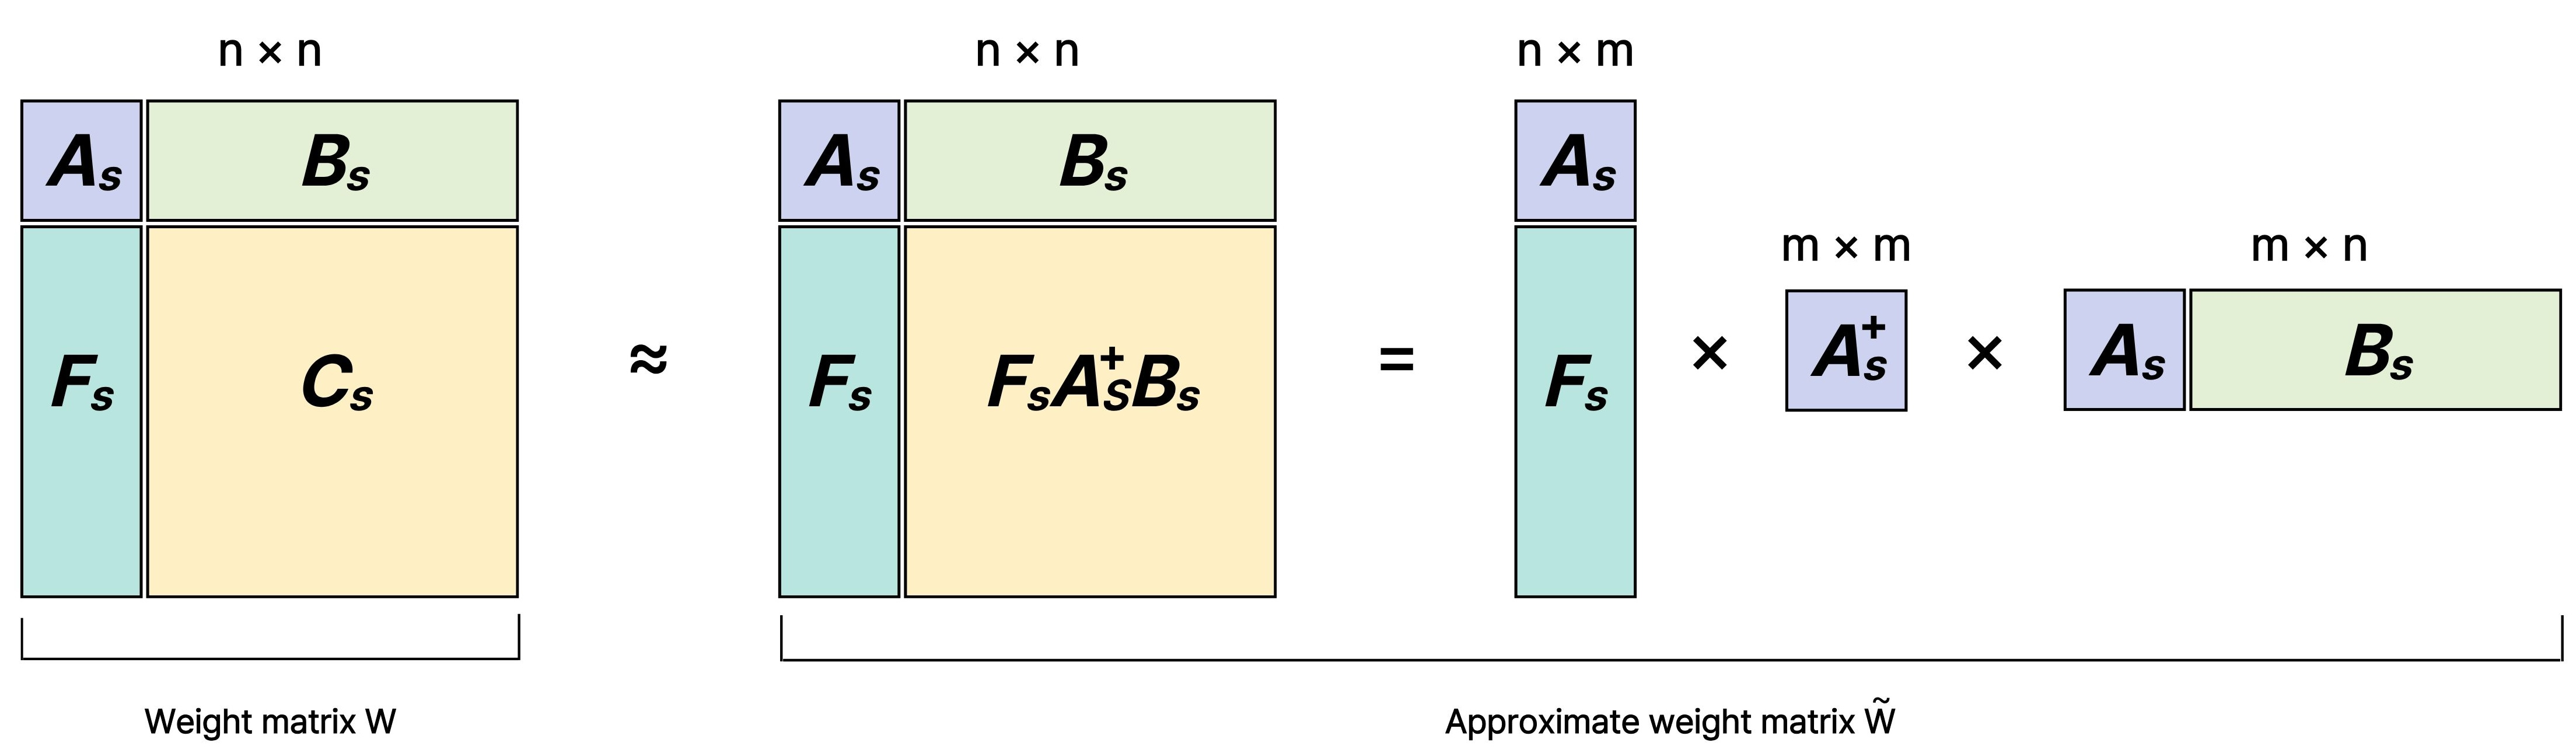
\includegraphics[width=\columnwidth]{../images/nystrom-approx.jpg}%
    }\\[6pt]
    \subfloat[Our \name{} Freivalds' check\label{fig:zkdiet}]{%
        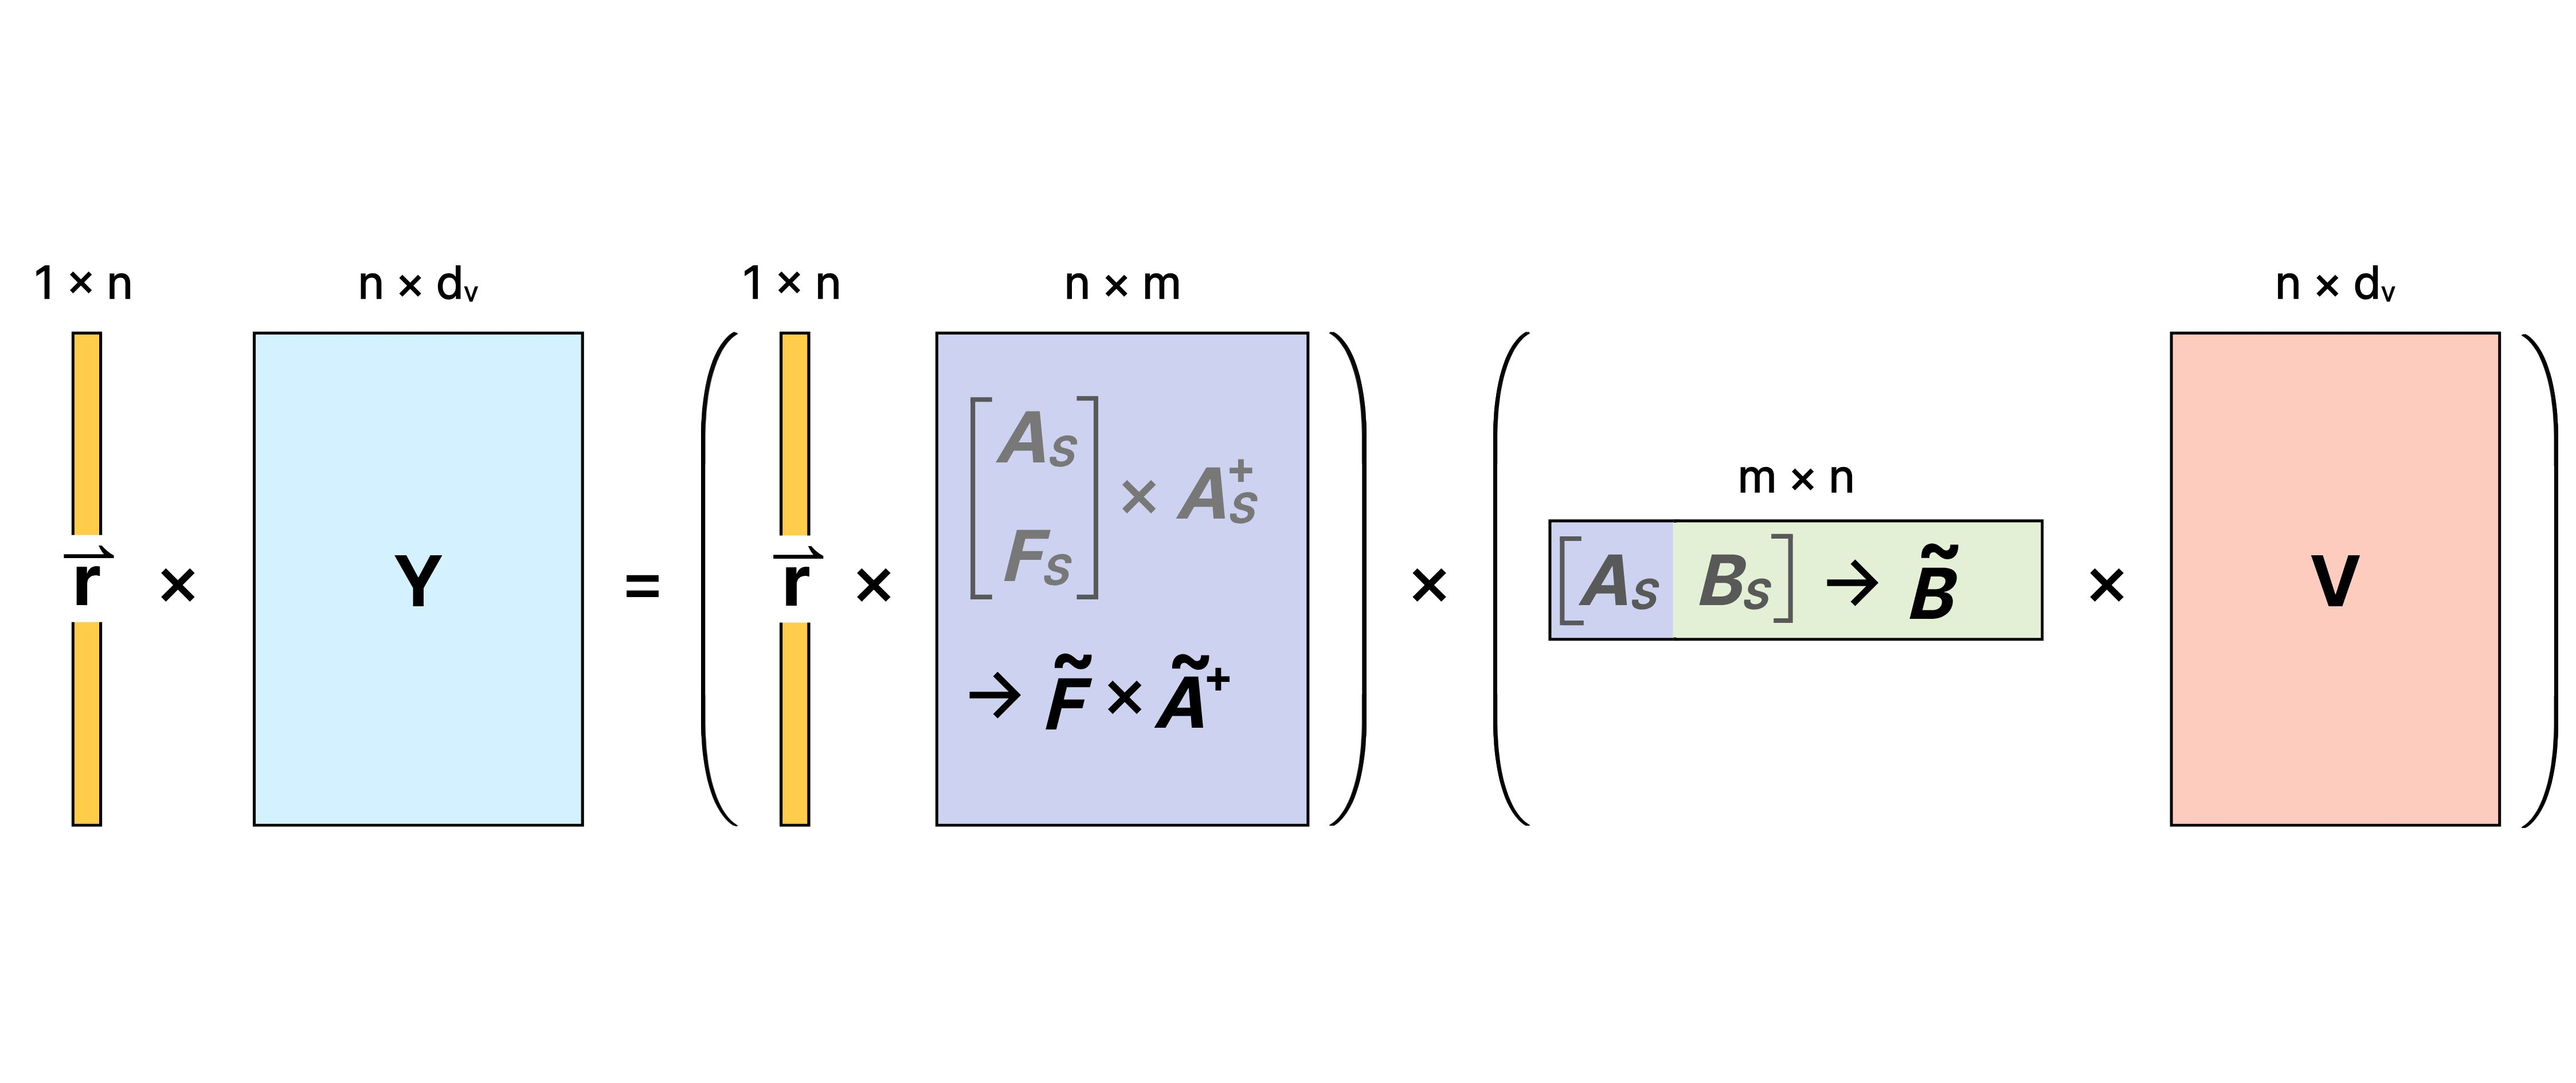
\includegraphics[width=\columnwidth]{../images/zkdiet-freivalds.jpg}%
    }
    \caption{Low-rank matrix multiplication with Freivalds' algorithm (illustrated for Nystr\"omformer). Other instances decompose the attention matrix differently (Table~\ref{tab:instance-comparison}).}
    \label{fig:chain}
\end{figure}

\paragraph{Low-rank factor chain.}
As illustrated in Figure~\ref{fig:nystrom-approx}, rather than directly handling the $n \times n$ self-attention matrix, we follow the Nystr\"omformer procedure and decompose it into a sequence of low-dimensional matrices of shapes $n \times m$, $m \times m$, and $m \times n$. We denote the three low-rank factors by
$\tilde{F} := \sfmax(\Q\widetilde{\K}^{\top}/\sqrt{d_k}) \in \mathbb{F}^{n \times m}$,
$\tilde{A} := \sfmax(\widetilde{\Q}\widetilde{\K}^{\top}/\sqrt{d_k}) \in \mathbb{F}^{m \times m}$, and
$\tilde{B} := \sfmax(\widetilde{\Q}\K^{\top}/\sqrt{d_k}) \in \mathbb{F}^{m \times n}$.
In the block decomposition of Figure~\ref{fig:nystrom-approx}, $\tilde{F}$, $\tilde{A}^{+}$, and $\tilde{B}$ take the roles of
$\bigl[\begin{smallmatrix} A_S \\ F_S \end{smallmatrix}\bigr]$,
$A_S^{+}$, and $\bigl[\, A_S \;\; B_S \,\bigr]$, respectively;
they are computed from the landmarks before the softmax rather than extracted from $S$ (cf.\ Section~\ref{subsec:lowrank}), so Figure~\ref{fig:zkdiet} is obtained from Figure~\ref{fig:nystrom-approx} by this substitution. The chain is thus $\Y = \tilde{F}\tilde{A}^{+}\tilde{B}\V$ with $G_1 = \tilde F$, $G_2 = \tilde A^{+}$, and $G_3 = \tilde B$.

\paragraph{Freivalds' checks.}
By applying Freivalds' algorithm to this low-rank representation (Figure~\ref{fig:zkdiet}), we compress the verification workload from $\mathcal{O}(n^2)$ to $\mathcal{O}(n)$, effectively reducing it to a chain of vector--matrix products of total size $2nm + m^2 + nd_v$: multiplying the random vector by $\tilde{F}$ ($nm$), then by $\tilde{A}^{+}$ ($m^2$), then by $\tilde{B}$ ($mn$), and finally by~$\V$ ($nd_v$). In the formal relation, this chain is verified in three fixed-point rescaled stages, with the two intermediate products committed (Section~\ref{moore-penrose}).

\paragraph{Non-linearities and the pseudoinverse witness.}
The softmax factors are enforced via lookup arguments. The pseudoinverse factor is instantiated by the iterative approximation $Z^{*}$ of Appendix~\ref{appx:newton-schulz}: the prover computes $Z^{*}$ outside the circuit and supplies it as a witness, and our protocol verifies in-circuit that $Z^{*}$ satisfies the Moore--Penrose conditions (Section~\ref{moore-penrose}) up to quantization tolerance. Since these conditions uniquely characterize the pseudoinverse $\tilde{A}^{+}$, this check constrains $Z^{*}$ to a small neighborhood of $\tilde{A}^{+}$, without ever computing $\tilde{A}^{+}$ itself.

\paragraph{Other instances.}
Linformer replaces the three-factor chain by two factors, $\Y = P\,(F\V)$ with $P = \sfmax(\Q(E\K)^{\top}/\sqrt{d_k})$, so the pseudoinverse step is absent and only one softmax is enforced. SOFT keeps the three-factor shape, $\Y = B A^{+} B^{\top}\V$, with a Gaussian-kernel lookup in place of softmax and the same pseudoinverse check. In all three cases the Freivalds projections, the lookup enforcement, and the commitment structure below are unchanged (Table~\ref{tab:instance-comparison}).

\begin{figure*}[!t]
    \centering
    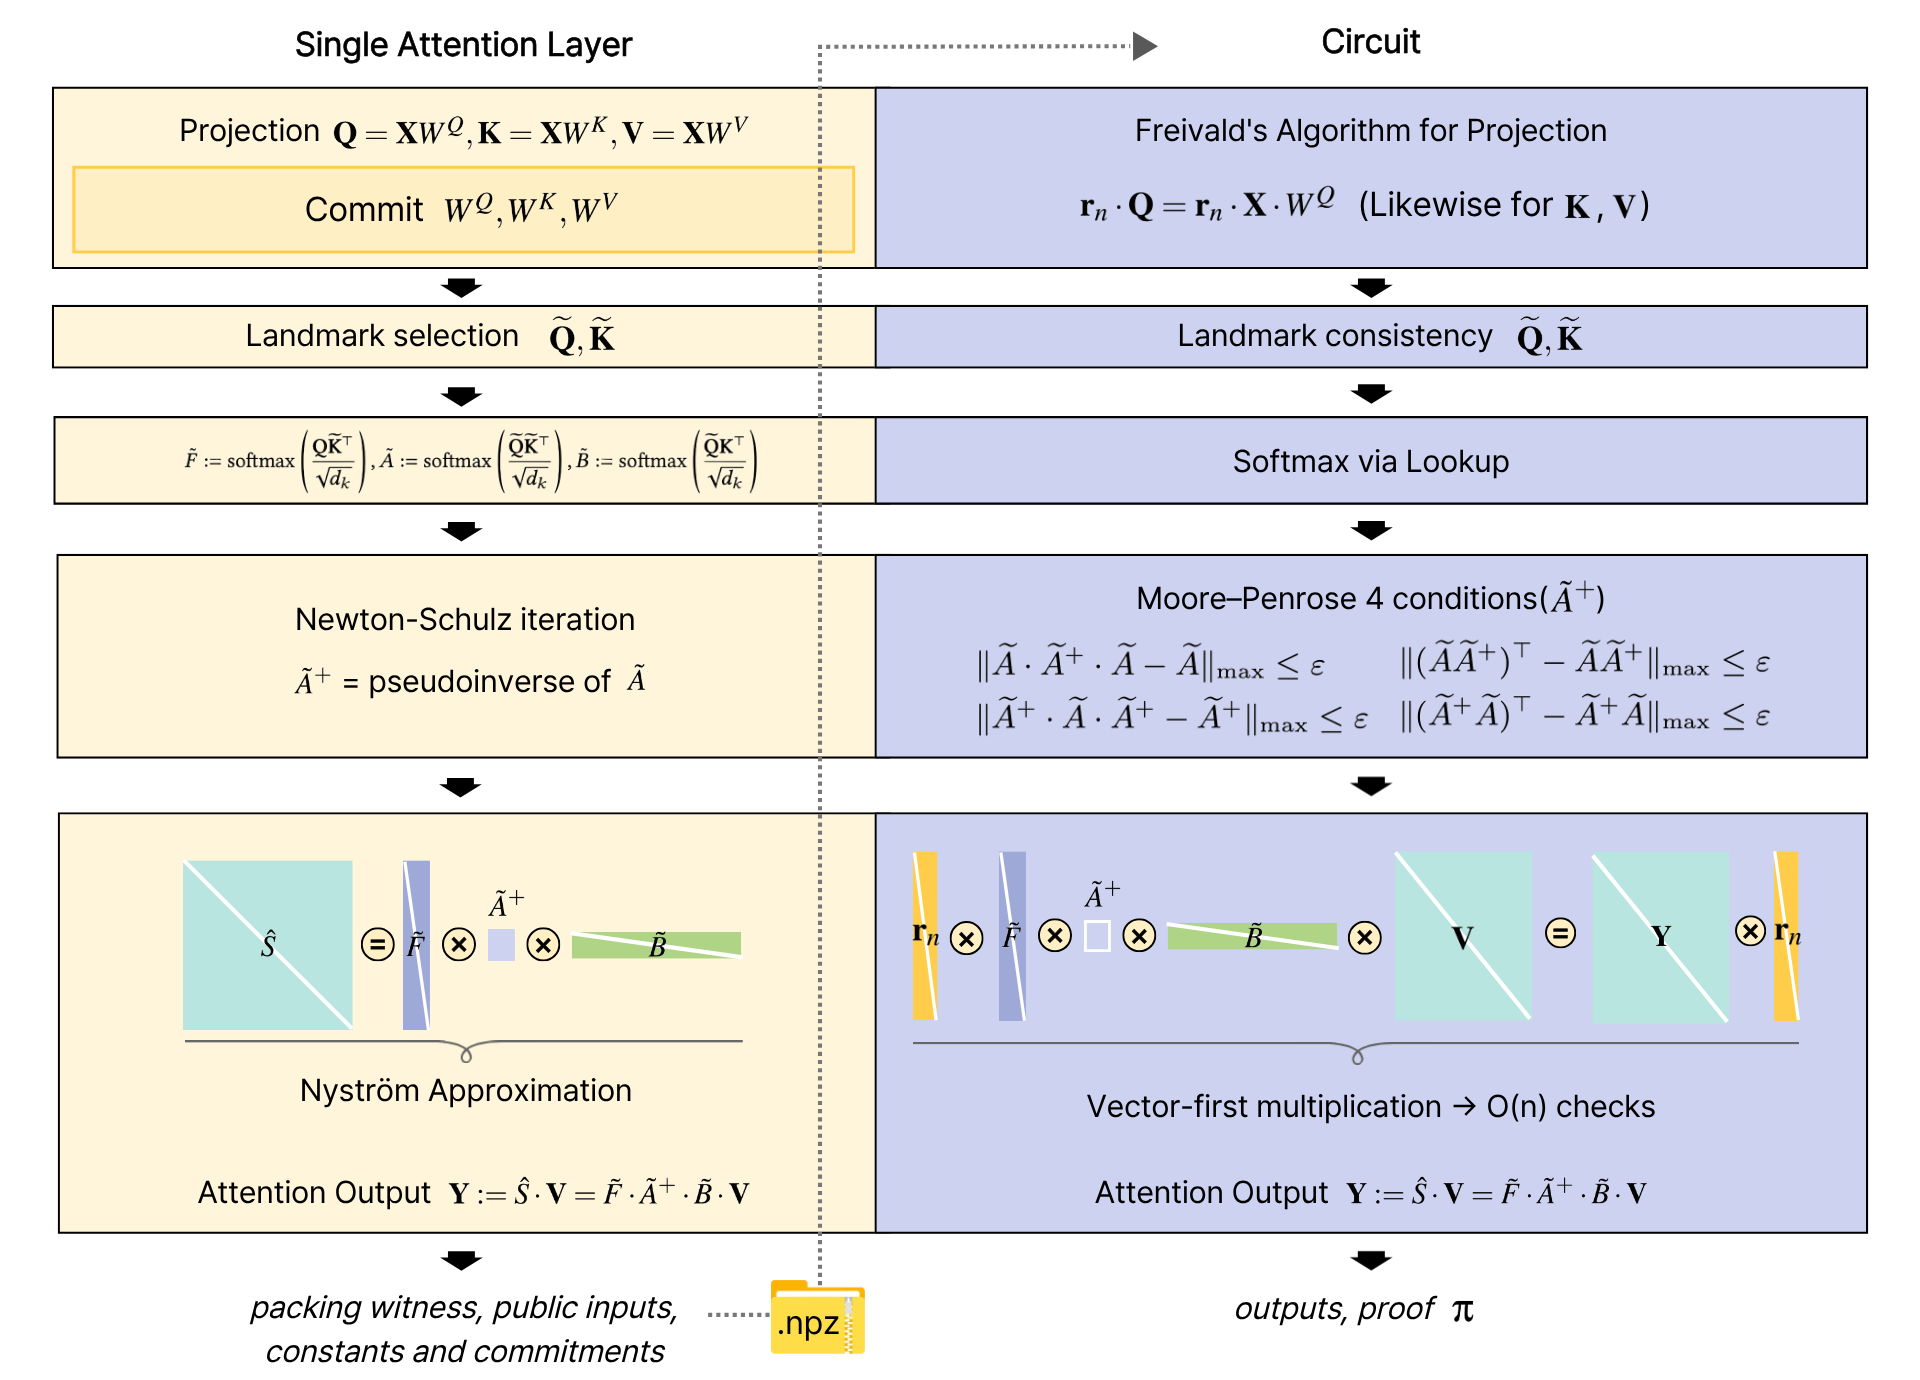
\includegraphics[width=0.9\textwidth]{../images/overview.png}
    \caption{Overview of Self-Attention and our framework}
    \label{fig:attention-overview}
\end{figure*}

\paragraph{Commit-carrying architecture.}
We embed these checks in a commit-carrying SNARK (CC-SNARK) architecture (Figure~\ref{fig:attention-overview}). Prior to serving any query, the provider publishes a global commitment $c_W \gets \Com.\commit(\ck_{\mathrm{glob}}, \W; o)$ to its weights under a circuit-independent key $\ck_{\mathrm{glob}}$.\footnote{For instances with $n$-dependent projection weights (e.g., Linformer), $c_W$ must be re-issued per sequence length; see Table~\ref{tab:instance-comparison}.} Each proof carries a circuit-dependent commitment linked to the global one via CP-linkage, so the verifier needs only constant-time checks.

For each query, the prover evaluates the attention pipeline locally, commits to the weights and intermediates under the circuit-dependent key $\ck$, sends commitments and output $\Y'$, and after receiving Freivalds challenges generates a composite proof $\pi$ encapsulating the CC-SNARK proof and two CP-linkages (Figure~\ref{fig:protocol}). In the non-interactive variant, challenges are derived via the Fiat--Shamir transformation after all commitments and $\Y'$ are fixed, preserving Freivalds' soundness.

Because zero-knowledge circuits operate over finite fields, we quantize all computations via the R1CS-friendly technique of~\cite{ZEN}. From this point onward, all matrices are over the finite field $\mathbb{F}$ after quantization.

\begin{figure*}[!t]
\centering
\newsavebox{\protocolbox}
\savebox{\protocolbox}{%
\fbox{\procedure[head=\textbf{Protocol (Nystr\"omformer instance)}, bodylinesep=2mm]{}{
        \mathcal{P}(\ck, c_W, \X; \{ \W^Q, \W^K, \W^V, \W^O\}) \< \< \mathcal{V}(\vk, c_W, \X) \\
        (\Y', \textit{aux}, \mathsf{lk}) \gets \NystromAttention(\X, \W^Q, \W^K, \W^V, \W^O) \\
        \widetilde{\cm}_{\W^i} \gets \Com.\commit(\ck,\W^i;\tilde{o}_i) \text{ for } i \in \{Q,K,V,O\} \\
        \widetilde{\cm} \gets \Com.\commit(\ck, \mathsf{lk} ;\tilde{o}) \\
        \widetilde{\cm}_{\mathsf{aux}} \gets \Com.\commit(\ck, (\Q,\K,\V,\tilde{A}^{+},\tilde{F}\tilde{A}^{+},\tilde{B}\V,\Y) ;\tilde{o}_{\mathsf{aux}}) \\
        \<  \sendmessageright*[2cm]{\{\widetilde{\cm}_{W^i}\}_{i \in \{Q,K,V,O\}}, \widetilde{\cm}, \widetilde{\cm}_{\mathsf{aux}}, \Y'\;} \< \\
        \< \sendmessageleft*[2cm]{\rand_n, \rand_m } \< \rand_n \sample \F^n, \t \rand_m \sample \F^m  \\
        \ins := (\X, \rand_n, \rand_m, \Y') \\
        \comwit := \{ (\W^i,\tilde{o}_i)_{i \in \{Q,K,V,O\}}, (\mathsf{lk}, \tilde{o}), (\Q,\K,\V,\tilde{A}^{+},\tilde{F}\tilde{A}^{+},\tilde{B}\V,\Y,\tilde{o}_{\mathsf{aux}}) \} \\
        \uncomwit := (\widetilde{\Q}, \widetilde{\K}, \Q\widetilde{\K}^{\top}, \widetilde{\Q}\widetilde{\K}^{\top}, \widetilde{\Q}\K^{\top}) \\
        \pi \gets \Pi_\mathsf{zkdiet}.\prove( \pk, \ins; (\comwit, \uncomwit)) \\
        \<  \sendmessageright*[2cm]\pi \< \\
        \< \< \Pi_\mathsf{zkdiet}.\verify(\vk, \ins, \{\widetilde{\cm}_{W^i}\}_{i \in \{Q,K,V,O\}},\, \widetilde{\cm}, \widetilde{\cm}_{\mathsf{aux}}, c_W, \pi)
    }}%
}%
\resizebox{0.9\textwidth}{!}{\usebox{\protocolbox}}
    \caption{Protocol message flow (Nystr\"omformer instance). The structure is identical for all instances; only the attention procedure and the committed/uncommitted witness partition differ.}
    \label{fig:protocol}
\end{figure*}

\paragraph{Commit Classification Principle.}
A matrix $M$ appearing in a Freivalds-projected identity requires pre-challenge commitment ($M \in \comwit$) if and only if no element-wise in-circuit constraint uniquely determines each entry of $M$ from already-committed data. Conversely, values recoverable entry-by-entry from committed data (e.g., pre-softmax logits from lookup index and remainder-limb decomposition, or segment-averaged landmarks from committed $\Q, \K$) need no separate commitment ($M \in \uncomwit$). Table~\ref{tab:instance-comparison} lists the $\comwit$ and $\uncomwit$ partition for each instance; the soundness argument of Section~\ref{sec:security-analysis} applies this classification uniformly.
